\documentclass{hfutpaper}
\usepackage[urlcolor=blue]{hyperref}
\usepackage{threeparttable}
\usepackage{setspace}
\usepackage{titlesec}
\usepackage{float}
\newcommand{\upcite}[1]{\textsuperscript{\textsuperscript{\cite{#1}}}}
\usepackage{fancyhdr}
\titleformat{\section}{\large \heiti}{\chinese{section}、}{0em}{}
\begin{document}
\begin{center}
\LARGE
  \textbf{标架及其在曲线和曲面理论中的应用}\\
  \vspace{0.2em}
  \large
    作者:王子 \ 学号:2016xxxxxx \\ %姓名,学号,班级
  专业班级:数学应用数学xx班
  \end{center}
\rule[0.1\baselineskip]{\textwidth}{0.5pt}
\textbf{摘 \ 要}\\
\large
微分几何是运用微积分的理论研究空间的几何性质的数学分支学科。
古典微分几何研究三维空间中的曲线和曲面,而现代微分几何开始研究更一般的空间——流形。
微分几何与拓扑学等其他数学分支有紧密的联系,对物理学的发展也有重要影响。爱因斯坦的广义相对论就以微分几何中的黎曼几何作为其重要的数学基础。
\\
\textbf{关键词}:厚德\quad 笃学\quad 崇实\quad 尚新\\
\rule[0.1\baselineskip]{\textwidth}{0.5pt}
\section{引言}
近代由于对高维空间的微分几何和对曲线、曲面整体性质的研究,使微分几何和拓扑学、变分学、李群理论等有了密切的关系,这些数学领域和微分几何互相渗透,已成为现代数学的中心课题之一。 
微分几何在力学和一些工程技术问题方面有广泛的应用,比如,在弹性薄壳结构方面,在机械的齿轮啮合理论应用方面,都充分应用了微分几何学的理论。


微分几何学的研究对数学其他分支以及力学、物理学、工程学等的影响是不可估量的。如:伪球面上的几何与非欧几何有密切关系;测地线和力学、变分学、拓扑学等有着深刻的联系,是内容丰富的研究课题。这方面有以J.阿达马、H.庞加莱等人为首的优异研究。极小曲面是和复变函数论、变分学、拓扑学关系极为深刻的研究领域,K.魏尔斯特拉斯、J.道格拉斯等人作出过卓越贡献。


微分几何学的研究工具大部分是微积分学。力学、物理学、天文学以及技术和工业的日益增长的要求则是微分几何学发展的重要因素。尽管微分几何学主要研究三维欧几里得空间中的曲线、曲面的局部性质,但它形成了现代微分几何学的基础则是毋庸置疑的。因为依赖于图形的直观性及由它进行类推的方法,即使在今天也未失其重要性。
\section{第一部分}
在曲面上有两条重要概念,就是曲面上的距离和角。比如,在曲面上由一点到另一点的路径是无数的,但这两点间最短的路径只有一条,叫做从一点到另一点的测地线。在微分几何里,要讨论怎样判定曲面上一条曲线是这个曲面的一条测地线,还要讨论测地线的性质等。另外,讨论曲面在每一点的曲率也是微分几何的重要内容。


在微分几何中,为了讨论任意曲线上每一点邻域的性质,常常用所谓“活动标形的方法”。对任意曲线的“小范围”性质的研究,还可以用拓扑变换把这条曲线“转化”成初等曲线进行研究。在微分几何中,由于运用数学分析的理论,就可以在无限小的范围内略去高阶无穷小,一些复杂的依赖关系可以变成线性的,不均匀的过程也可以变成均匀的,这些都是微分几何特有的研究方法。


合肥工业大学是中华人民共和国教育部直属全国重点大学,教育部、工信部和安徽省政府共建高校,国防科工局与教育部共建高校。学校创建于1945年,1960年被中共中央批准为全国重点大学。刘少奇、朱德、董必武、陈毅、邓小平等老一辈无产阶级革命家先后来校视察指导工作,邓小平同志在1979年亲笔为学校题写了校名。2005年成为国家“211工程”重点建设高校,2009年成为国家“985工程”优势学科创新平台建设高校,2017年进入国家“双一流”建设高校行列。
学校在安徽省省会合肥市设有屯溪路校区、翡翠湖校区、六安路校区和合肥工业大学智能制造技术研究院,在安徽省宣城市设有合肥工业大学宣城校区。学校先后荣获第四届全国文明单位和首届“全国文明校园”等多个荣誉称号\upcite{bib:one}。
\begin{table}[H]
	\caption{表格}
	\centering
	\begin{tabular}{cccccccc}
		\toprule[1.5pt]
		年份  & 2006&2007&2008&2009&2010 & 2011 & 2012 \\
		\midrule
		A&57.95&58.187&59.1&59.652&60.22&61.072&61.418 \\
		B &55.7957 &58.3199&58.8548&59.9983&60.3769 &60.9841 &61.7716 \\		
		C&2.1543&0.1329&0.2452&0.3463&0.1569&0.0879&0.3536 \\		
		D&0.0372 &0.0023&0.0041&0.0058&0.0026&0.0014&0.0058 \\
		\bottomrule[1.5pt]
		\label{tab1}
	\end{tabular}
\end{table}
\section{第二部分}
在合肥,“吃在工大”的美名,一直在各高校之间传递。这是学校饮食服务战线全体职工数十年来共同努力的结果。为了让来自全国各地的同学在学校感受到家的温暖,食堂经理赵冬生所在的食堂推出了一项“点餐墙”的服务。同学们想吃家乡菜了,可以在食堂点餐墙上留下字条,食堂的厨师们会根据留言,为同学们“量身定做”家乡菜。项服务一经推出,就深受同学们的欢迎,每天点餐墙上的字条都有好几十份。但这也让赵冬生感到“压力山大”。不久前,一位来自东北的同学在点餐墙上留言想吃家乡的锅包肉,但赵冬生和同事们做出的菜却总不能让学生满意。于是,赵冬生带上厨师特地去东北餐馆学艺。“经过反复尝试,点餐的同学终于高兴地说,吃上了真正的家乡味。”。
\begin{figure}[H]%H表示图强制在下面,想设置浮动环境用htp
	\centering  %插入的图片居中表示
	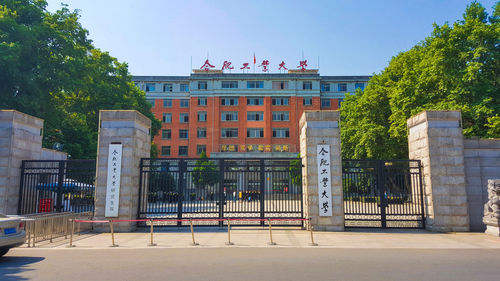
\includegraphics[scale=0.5]{hfut}  %插入的图,包括JPG,PNG,PDF,EPS等,放在源文件目录下
	\caption{主教大楼}  %图片的名称
	\label{fig1}
\end{figure}
据统计,每年从合肥工业大学毕业的上万名毕业生,近75\%服务于国家装备制造业及建筑、能源、信息等重点工程和项目领域,其中本科毕业生到世界500强和中国500强企业工作和硕士毕业生到国有企业研发中心、科研院所、高等学校工作的均占签约就业总数的65\%。毕业生对就业状况满意度和用人单位对毕业生满意度均超过95\%\upcite{bib:two}
\begin{thebibliography}{9}%宽度9
\bibitem{bib:one} 毕郑南.陈省身在数学领域的独特人生[J].兰台世界,2014,(4):68-69.
\bibitem{bib:two} 王永青,刘海波,贾振元, 等.基于活动标架理论的加工目标曲面再设计及刀位计算[J].机械工程学报,2012,48(19):141-147. 
\end{thebibliography}
\section*{matlab源程序}
\begin{lstlisting}[language=matlab]
clc;clear;
row = size(A) 
row = size(A,1) 
column = size(A,2) 
[row,column] = size(A) 
\end{lstlisting}
\end{document} 